%!TEX root = ../thesis.tex
\markboth{Appendix}{APPENDIX}
\begin{appendices}

% \renewcommand\thetable{A.\arabic{table}}
\setcounter{figure}{0}
\setcounter{table}{0}

\addcontentsline{toc}{chapter}{Appendices}

% ---------------------------------------------------------------

\addcontentsline{toc}{section}{A. Materials for the MixT Formative Study}
\subsection{Appendix A. Materials for the MixT Formative Study}
\label{mixt_formative_tutorial2}

The complete tutorial of Task 2 we provided in the MixT formative study.

\vspace{20pt}
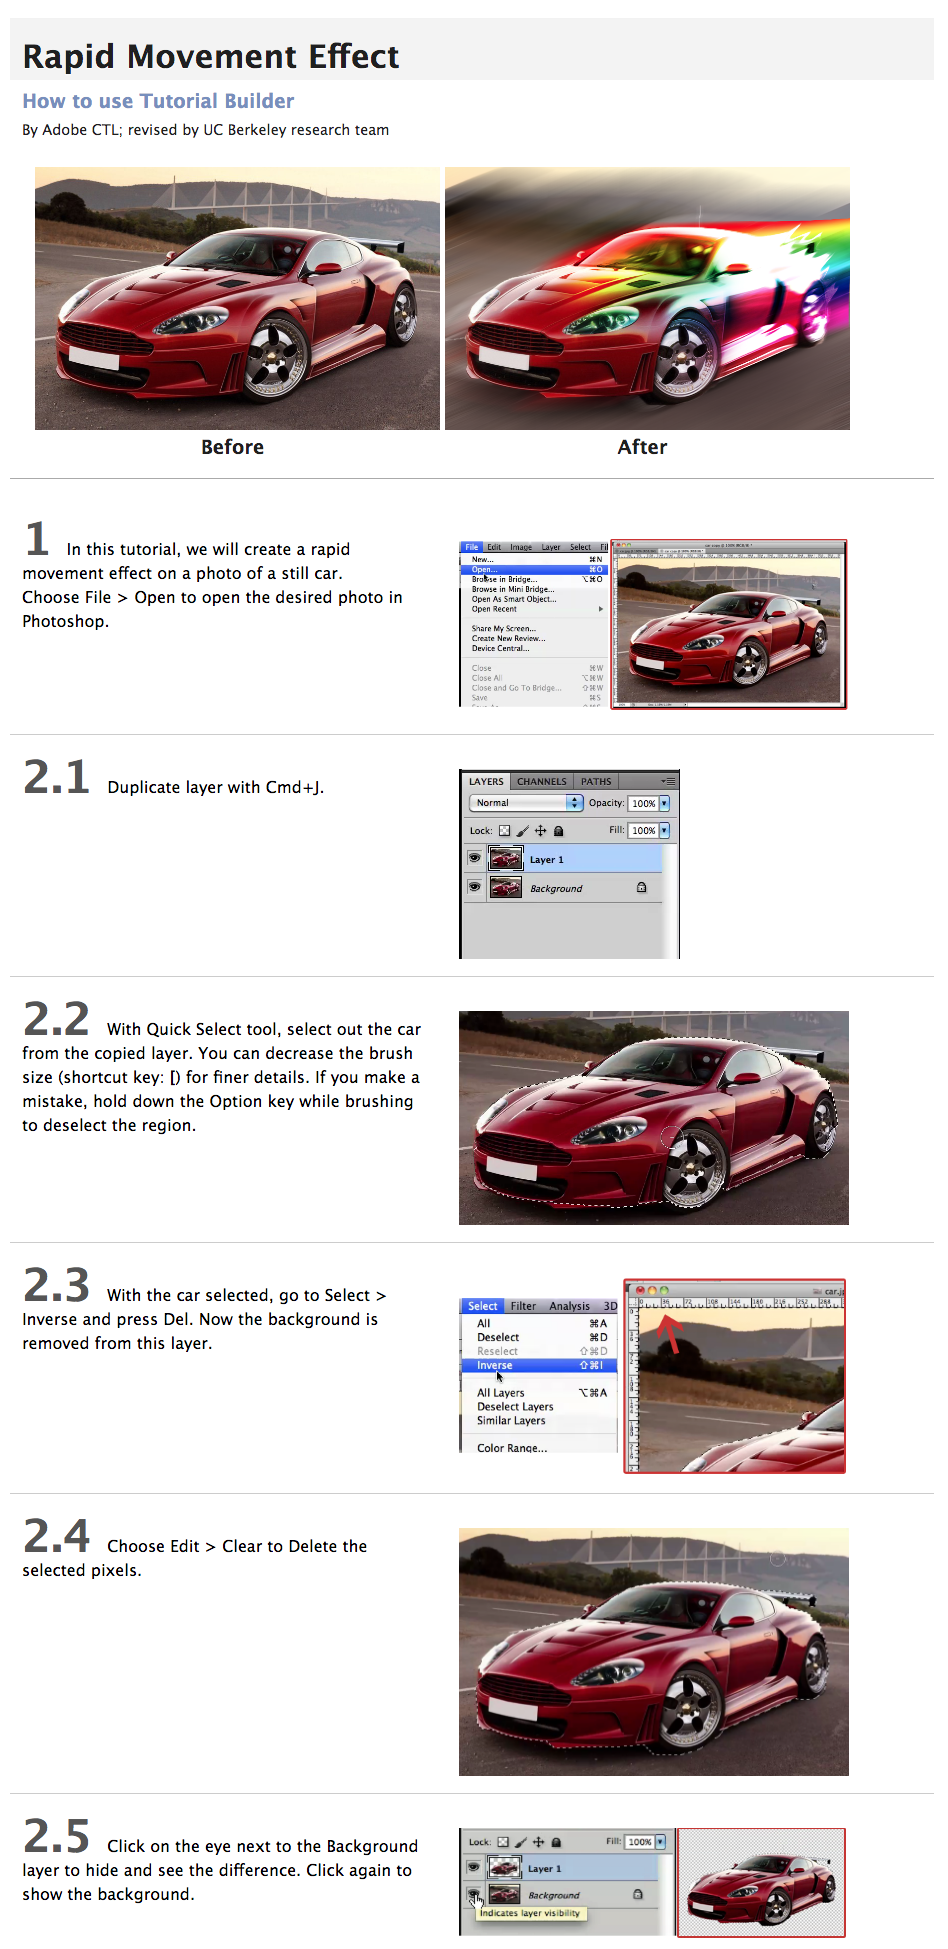
\includegraphics[width=0.495\textwidth]{\mixt/fig/formative_study/tutorial2/car_complete1}
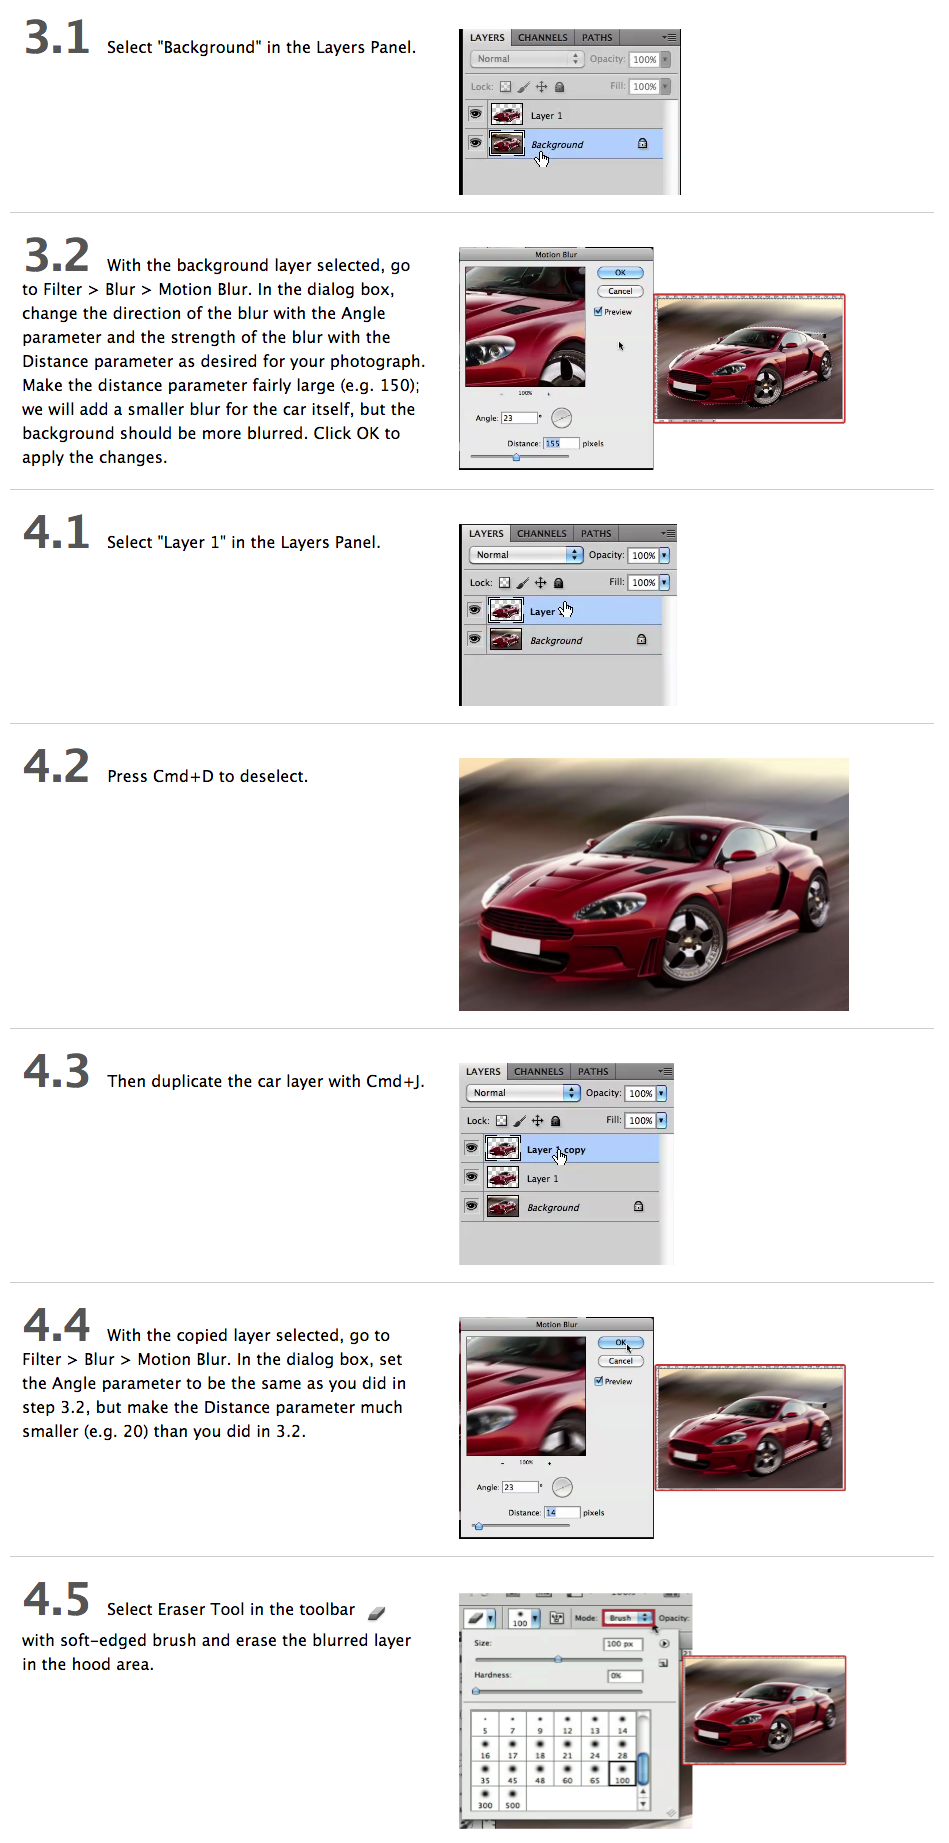
\includegraphics[width=0.495\textwidth]{\mixt/fig/formative_study/tutorial2/car_complete2}

\clearpage

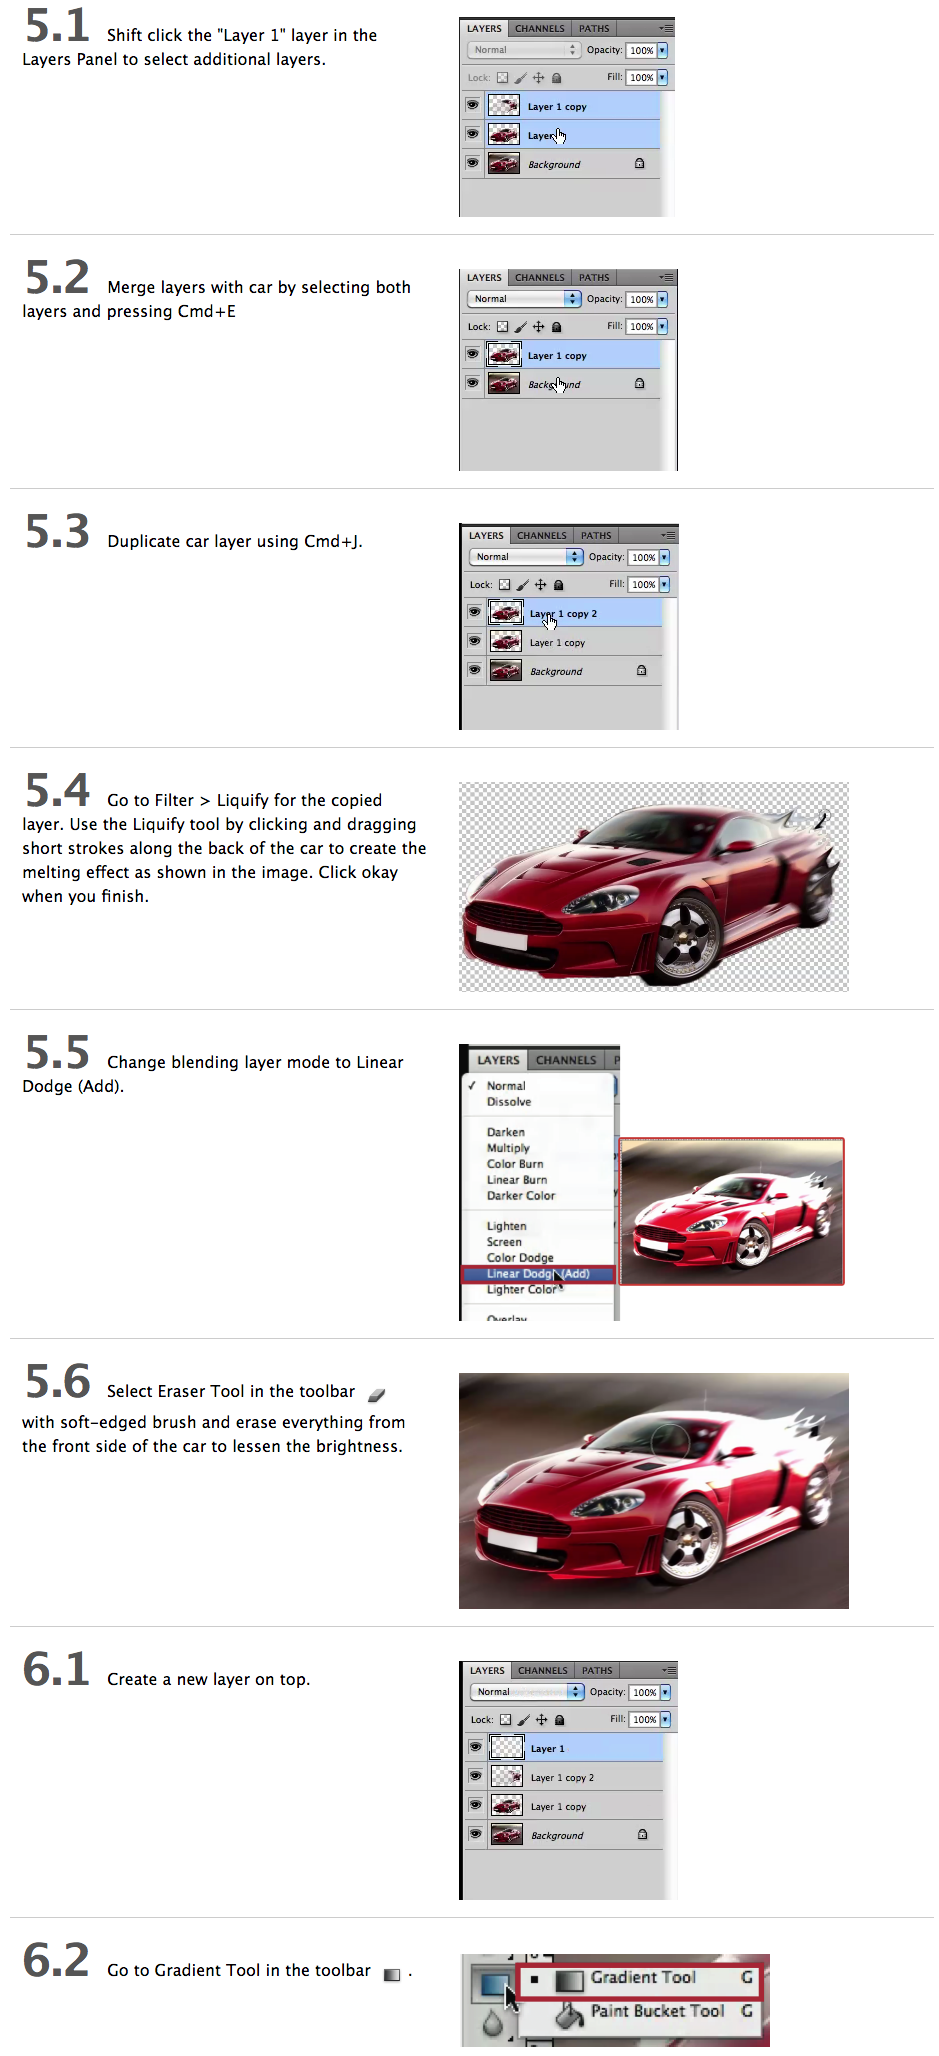
\includegraphics[width=0.495\textwidth]{\mixt/fig/formative_study/tutorial2/car_complete3}
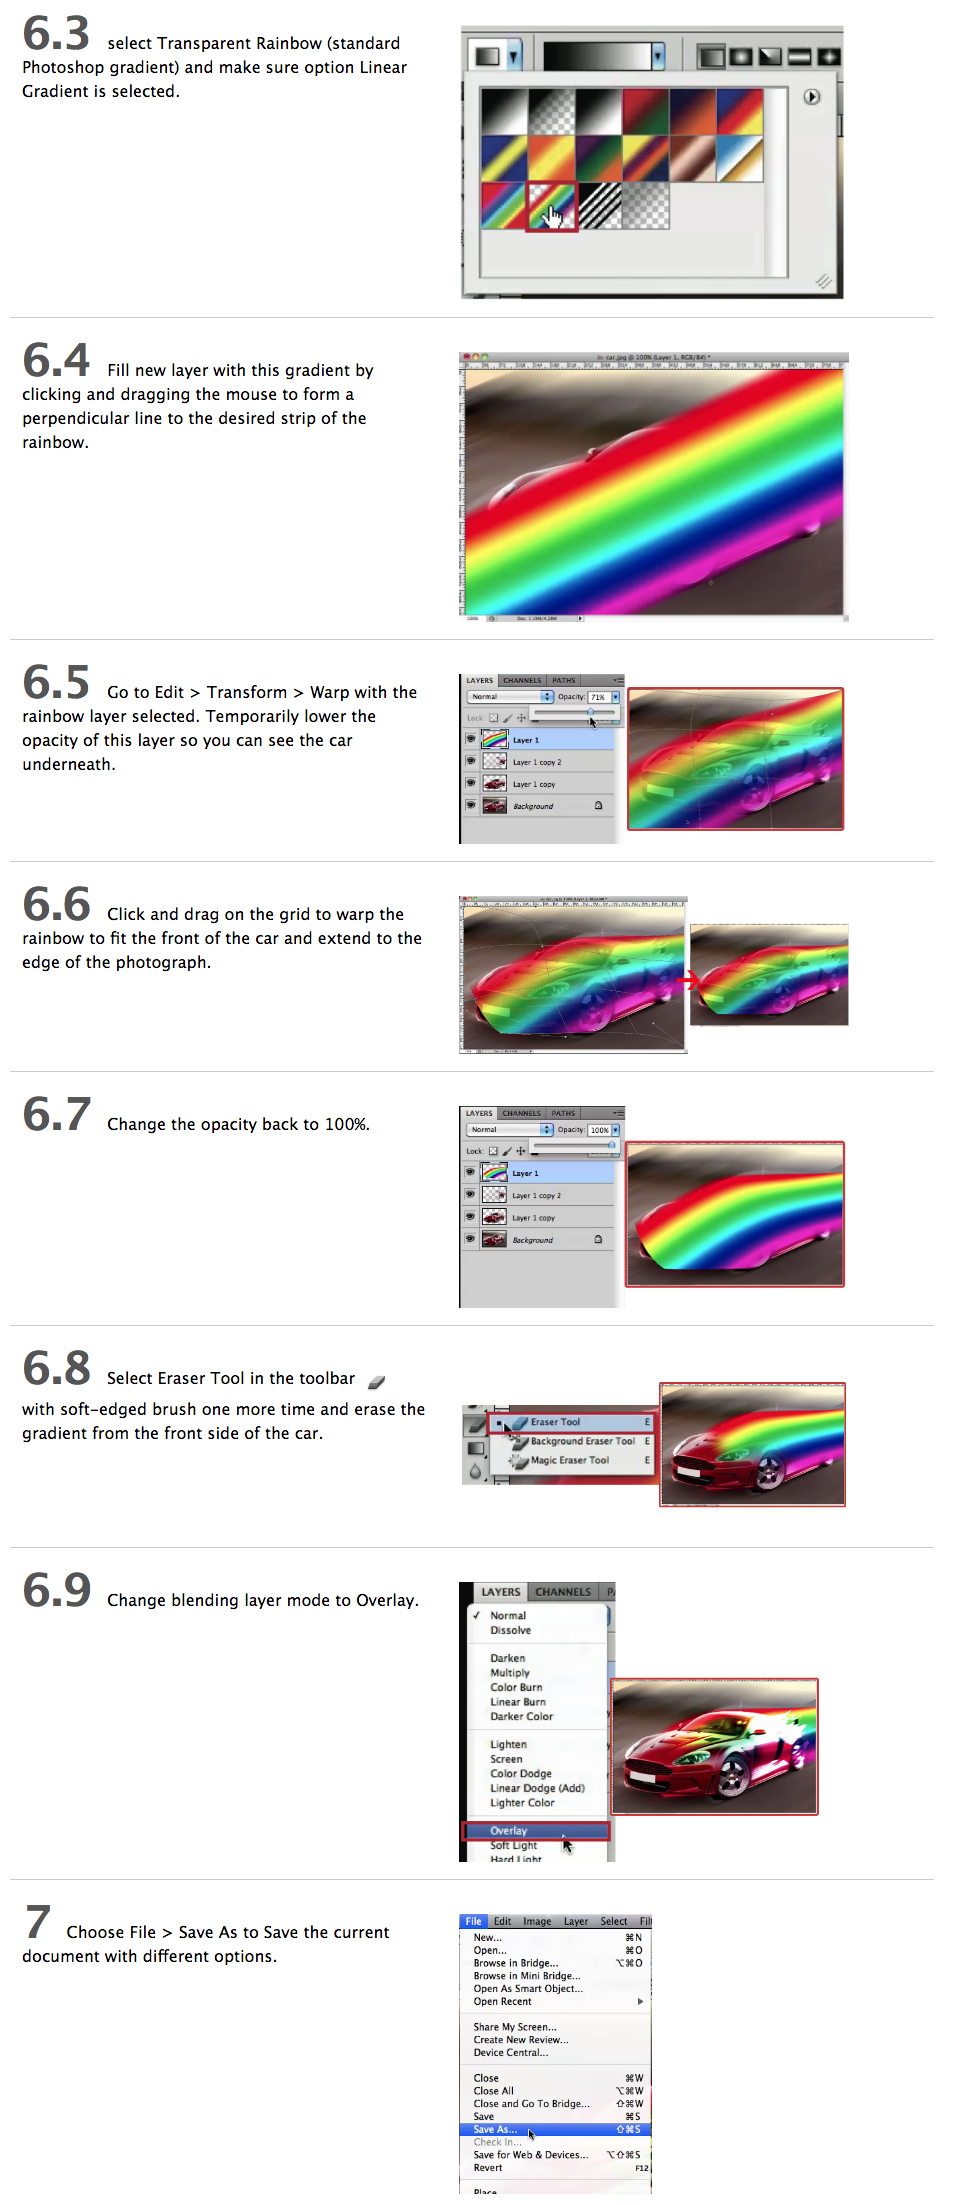
\includegraphics[width=0.495\textwidth]{\mixt/fig/formative_study/tutorial2/car_complete4}

\clearpage

% ---------------------------------------------------------------

\addcontentsline{toc}{section}{B. Materials for the DemoCut Formative Study}
\subsection{Appendix B. Materials for the DemoCut Formative Study}
\label{democut_formative}

20 YouTube How-To videos we analyzed in the DemoCut formative user study.\\
A video playlist is available online at\\
\url{https://www.youtube.com/playlist?list=PLAq2QZEiIgn80wbHOp9In4s8IzDnkb3II}

\vspace{20pt}
\noindent
\begin{minipage}[b]{1.0\textwidth}
  \noindent
  \footnotesize
\begin{tabular}{| l | r | l | r | r | l |}
    \hline
  Category & Index & Length & Views & Creation Date & Link\\ \hline
Electronics & 1 & 1:54:00 & 3,006  & Oct 21, 2012  & \url{https://youtu.be/watch?v=zOBy6iKjpso} \\
  & 2 & 5:32:00 & 22,211 & Sep 16, 2012  & \url{https://youtu.be/watch?v=4cuneFm-AG4} \\
  & 3 & 6:00:00 & 71,895 & Jun 18, 2012  & \url{https://youtu.be/watch?v=hOdu1Zl1lic} \\
  & 4 & 5:34:00 & 130,001  & Jun 30, 2011  & \url{https://youtu.be/watch?v=zYjOqcbBEco} \\ \hline
Home/Repair & 5 & 5:59:00 & 2,231  & Oct 6, 2012 & \url{https://youtu.be/watch?v=Y5j55Mlg09s} \\
  & 6 & 8:40:00 & 5,063  & Jan 4, 2013 & \url{https://youtu.be/watch?v=54k_OgAT_uQ} \\
  & 7 & 3:42:00 & 8,312  & Mar 15, 2011  & \url{https://youtu.be/watch?v=JL5Q2lJAAdk} \\
  & 8 & 7:28:00 & 32,201 & Mar 10, 2012  & \url{https://youtu.be/watch?v=7OrXrmFqXv0} \\ \hline
Art & 9 & 5:50:00 & 699,177  & April 12, 2012  & \url{https://youtu.be/watch?v=RFauBl0zTvw} \\
  & 10  & 4:53:00 & 4,004,613 & Nov 18, 2011  & \url{https://youtu.be/watch?v=iybQwiJWToM} \\
  & 11  & 9:08:00 & 58,248 & Aug 27, 2012  & \url{https://youtu.be/watch?v=va0sOYEHRho} \\
  & 12  & 2:26:00 & 6,203  & Feb 8, 2013 & \url{https://youtu.be/watch?v=NHfPywNg_Vw} \\ \hline
Craft & 13  & 6:25:00 & 12,8741  & Jan 12, 2013  & \url{https://youtu.be/watch?v=RajOsFVWJ4I} \\
  & 14  & 3:09:00 & 19,303 & Jan 22, 2013  & \url{https://youtu.be/watch?v=8KP-trX9I5g} \\
  & 15  & 4:17:00 & 1,156  & Oct 5, 2012 & \url{https://youtu.be/watch?v=ajW6h6JAR04} \\
  & 16  & 2:32:00 & 2,804  & Feb 2, 2013 & \url{https://youtu.be/watch?v=qBUJtRNUGOA} \\ \hline
Food  & 17  & 2:16:00 & 130,752  & Jun 4, 2009 & \url{https://youtu.be/watch?v=3opfBL9YZ10} \\
  & 18  & 8:14:00 & 30,740 & Apr 11, 2011  & \url{https://youtu.be/watch?v=DWxUa9LwbSY} \\
  & 19  & 3:47:00 & 22,670 & Sep 12, 2011  & \url{https://youtu.be/watch?v=l0QHDHMe9oU} \\
  & 20  & 3:54:00 & 9,192  & Feb 6, 2012 & \url{https://youtu.be/watch?v=5G3OGIN7Cx8} \\ \hline
\end{tabular}
\end{minipage}

\clearpage

% ---------------------------------------------------------------

\addcontentsline{toc}{section}{C. The Initial Design of Kinectograph}
\subsection{Appendix C. The Initial Design of Kinectograph}
\label{kinectograph_original_design}

The initial design of Kinectograph and its hardware components that we used in Study 1 and 2. A base (c) stabilizes the system and houses the electronics, such as a custom PCB board (b). The bottom servo (a) of the pan-tilt system fastens to the middle of the base, while the Kinect holder (d) attaches the Kinect sensor to the pan-tilt system. Both (c) and (d) are fabricated on a Projet HD 3000 printer.

\centering
\vspace{20pt}
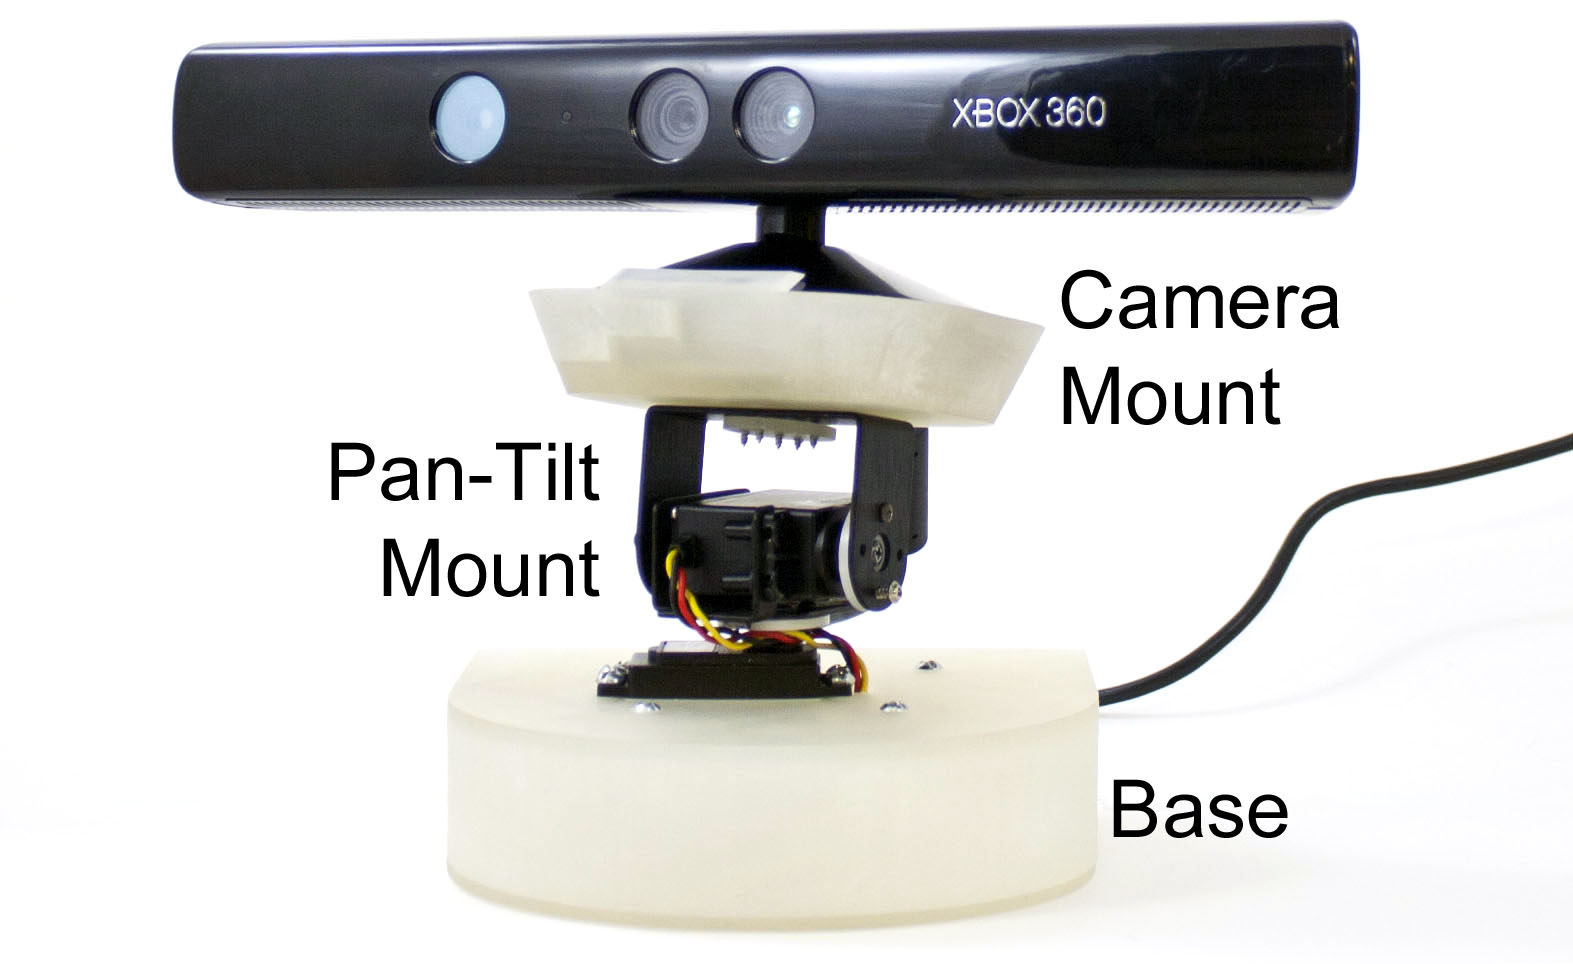
\includegraphics[width=0.5\columnwidth]{\kinectograph/fig/device-annotated}
\vspace{20pt}
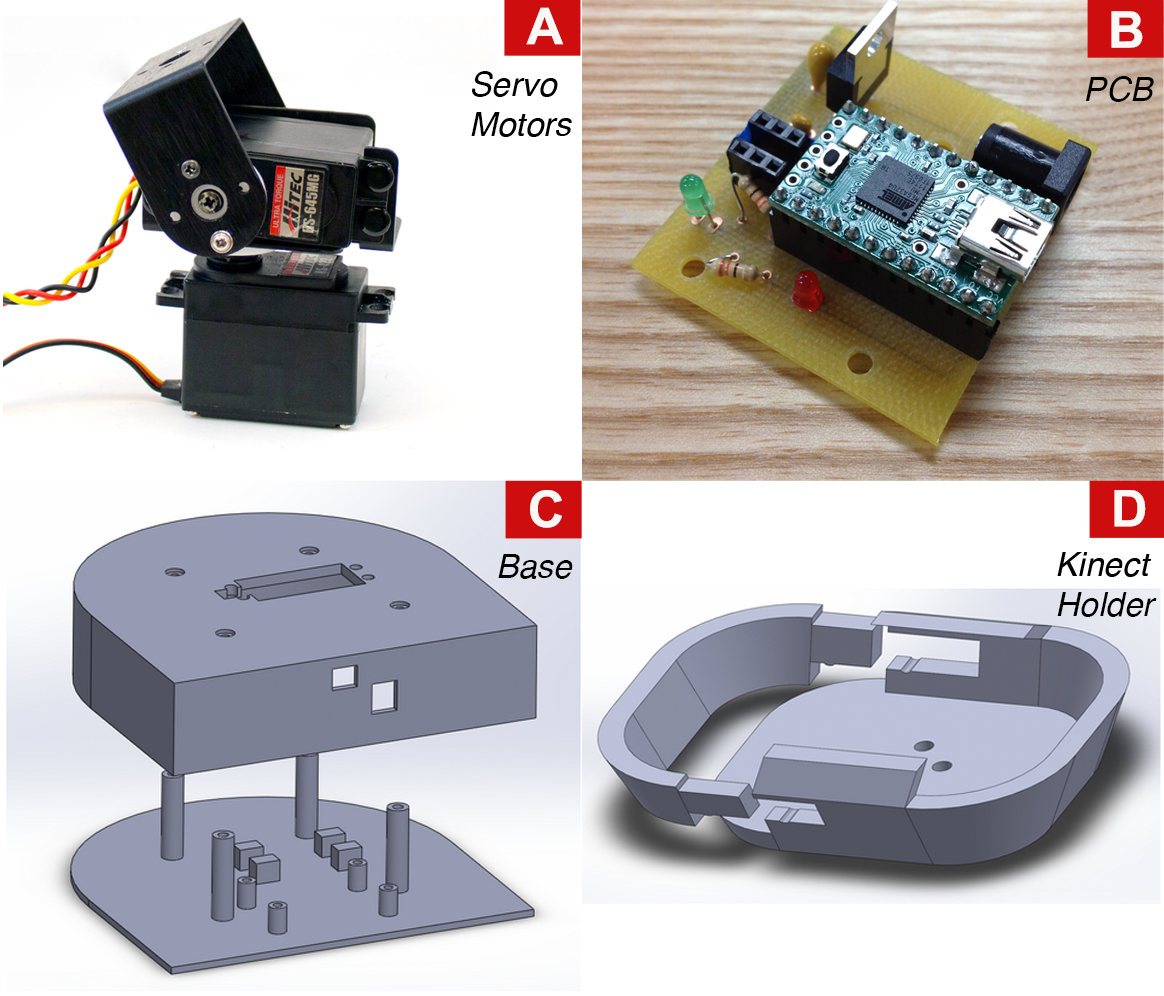
\includegraphics[width=0.55\columnwidth]{\kinectograph/fig/components_new}

\clearpage

% ---------------------------------------------------------------

\addcontentsline{toc}{section}{D. Materials for the DemoDraw User Study and Selected Results}
\subsection{Appendix D. Materials for the DemoDraw User Study and Results}
\label{demodraw_study_materials}

\renewcommand\thefigure{D.\arabic{figure}}

\begin{figure}[h!]
     \centering
    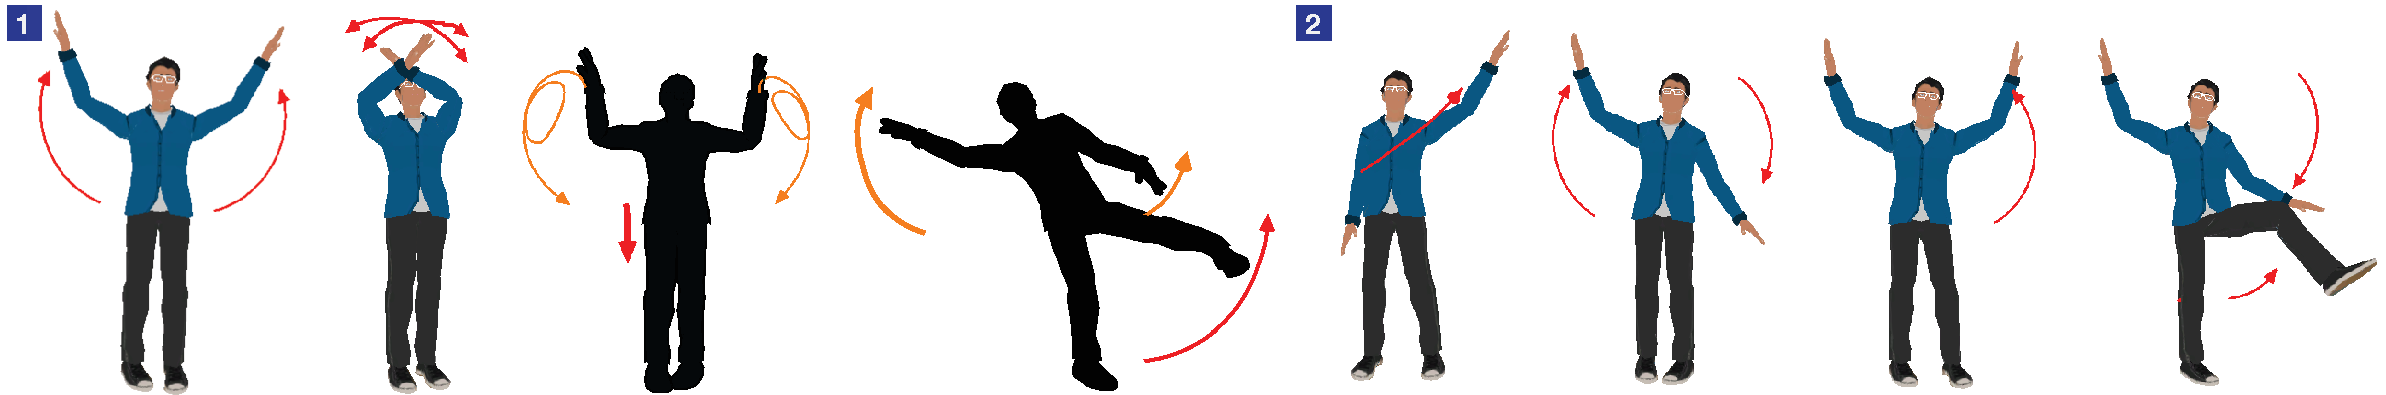
\includegraphics[width=\columnwidth]{\demodraw/fig/study1/study1_tasks}
    \caption{Tasks provided in Study 1: We showed the printouts of these two sets of 4-step motions generated by DemoDraw using both the Demonstration Interface and the Refinement Interface. We asked participants to re-perform in front of a camera.}
    \label{fig:study_review_tasks}
 \end{figure}

   \vspace{6mm}
\begin{figure}[h!]
     \centering
    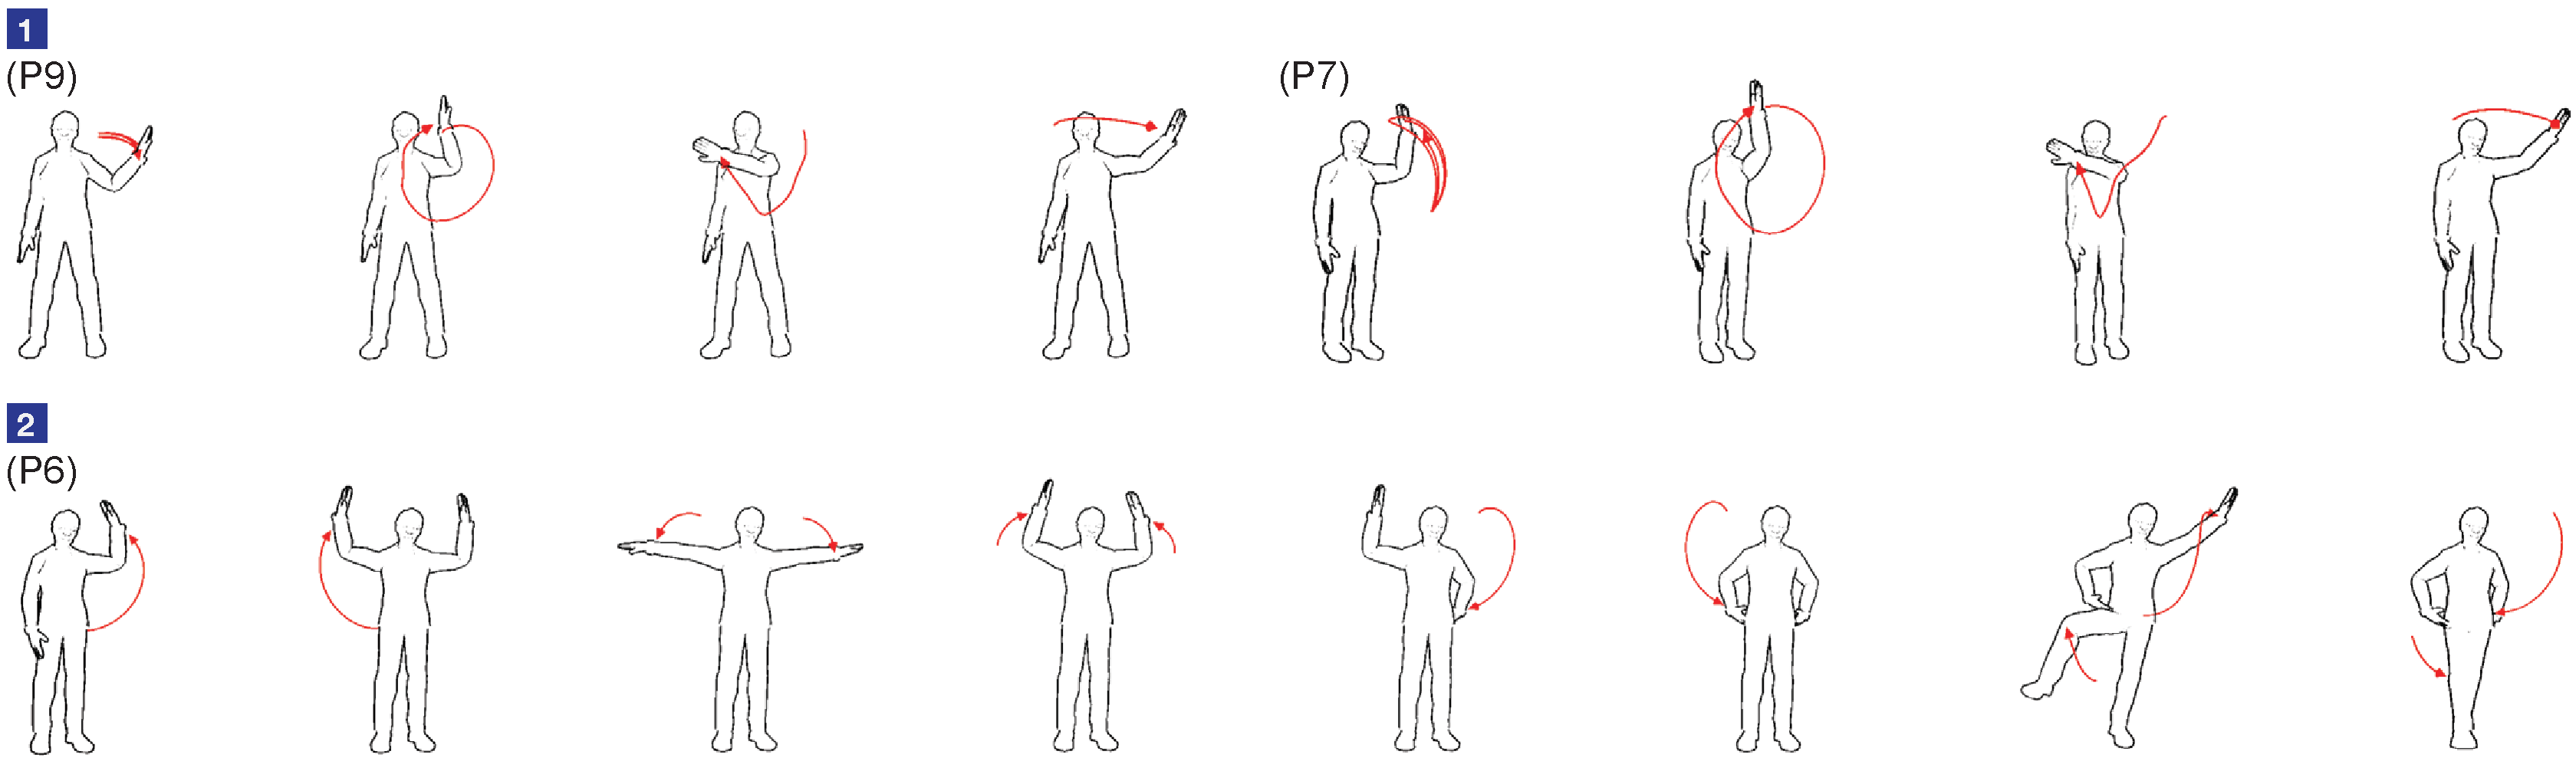
\includegraphics[width=\columnwidth]{\demodraw/fig/study2/study2_tasks}
    \caption{Step-by-step illustrations generated by participants in Study 2 using the \phaseI{}: 1) Results from P9 and P6 showing the same four gestures of a gestural interface in task 1, and 2) Results from P6 showing 8-step moves in task 2.}
    \label{fig:study_authoring_tasks}
   \end{figure}

\begin{figure}[h!]
     \centering
    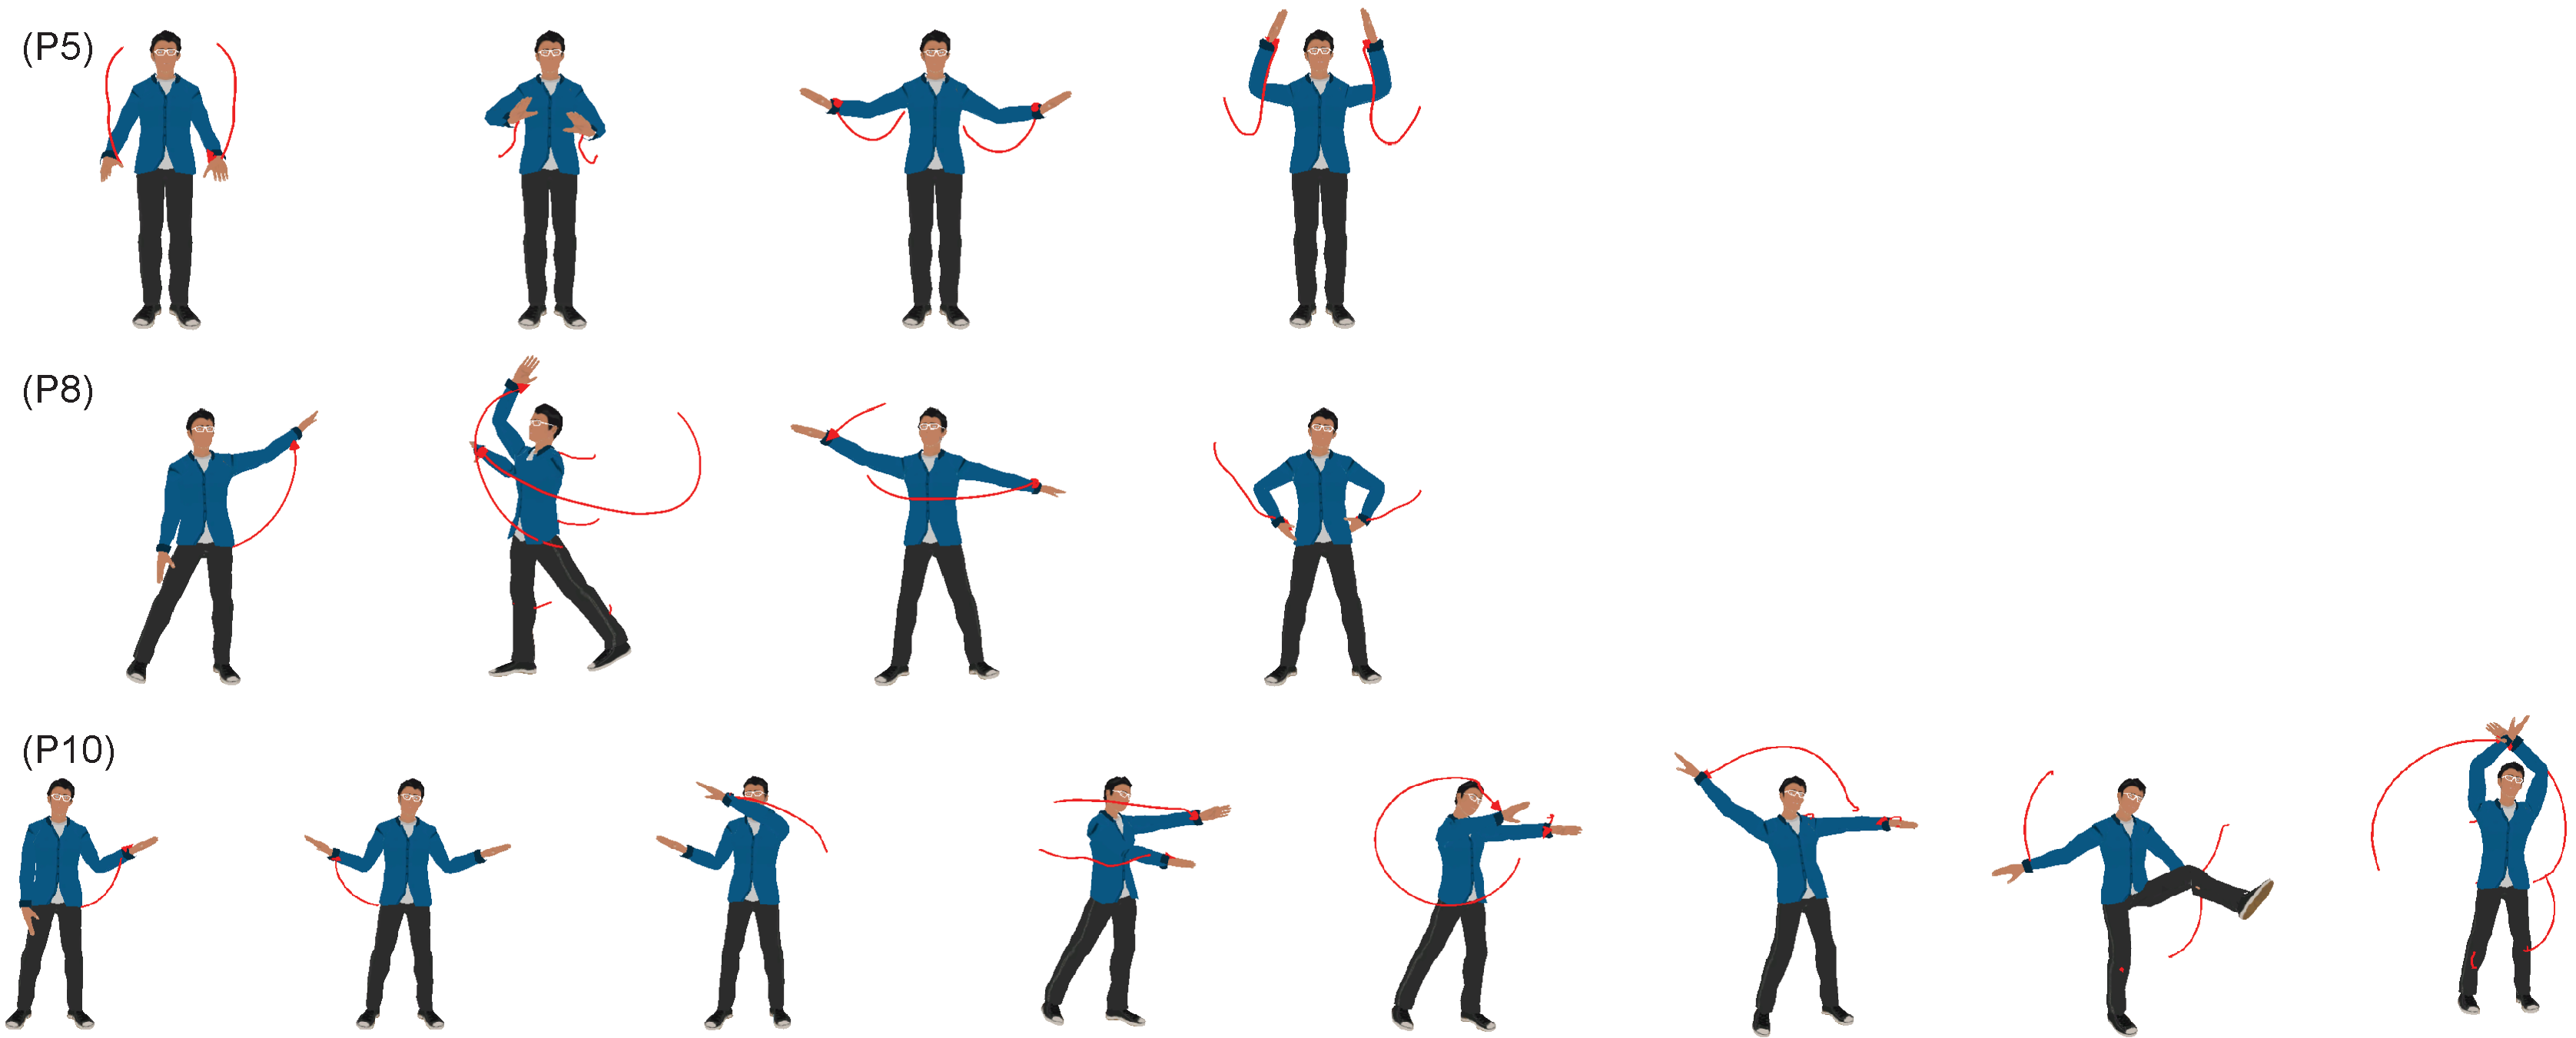
\includegraphics[width=\columnwidth]{\demodraw/fig/study2/study2_open}
    \caption{Selected illustrations from the open-ended task created by three different participants using the using Demonstration Interface in Study 2: P5 performed to conduct a 4/4 beat pattern; P8 and P10 each performed four and eight free moves.}
    \label{fig:open_ended_examples}
 \end{figure}

\end{appendices}
